\chapterimage{img/SuperKK.jpg} % Chapter heading image
\chapterspaceabove{6.75cm} % Whitespace from the top of the page to the chapter title on chapter pages
\chapterspacebelow{7.25cm} % Amount of vertical whitespace from the top margin to the start of the text on chapter pages

%------------------------------------------------

\chapter{Introduzione}\index{Introduzione}

In questo capitolo vengono introdotti i contenuti e le finalità del corso. Vengono inoltre introdotti i concetti base del corso.


\section{Informazioni sul corso e finalità}\index{Finalità del corso}

Si riporta dalla pagina \href{https://elearning.df.unipi.it/course/view.php?id=237}{e-learning} del corso la finalità di questo esame:
\begin{quote}
    Nella prima parte del corso lo studente dovrà acquisire una certa conoscenza delle principali caratteristiche dei raggi cosmici e dei metodi utilizzati per la loro rilevazione, conoscenze sui recenti sviluppi nelle misure e rivelazione di neutrini dal sole, conoscenza molto elementare della relatività generale e di come derivare le equazioni di Friedmann-Lemaitre, conoscenza di base dei modelli cosmologici standard, dei suoi limiti e dei possibili candidati alla materia oscura, conoscenza dei metodi di rivelazione sperimentale diretta e indiretta di candidati materia oscura. 
    Nella seconda parte del corso si richiede allo studente di acquisire una conoscenza di base della teoria e della rivelazione delle onde gravitazionali.
\end{quote}

\section{Introduzione storica}\index{Introduzione!Introduzione storica}

Cominciamo studiando la storia dei raggi cosmici. Le prime ipotesi risalgono a Charles Coulomb, che nel 1785 osservò con un elettroscopio a foglie che questo si scaricava spontaneamente nel tempo: ciò portò all'ipotizzazione di una carica presente nell'aria circostante. Studi successivi di Hess e Kolhörster misurano (con l'uso di palloni aerostatici) l'aumento della capacità ionizzante di questo \emph{qualche cosa} con l'aumentare dell'altitudine. Il fisico statunitense Millikan confermò con i suoi studi l'orignie extraterrestre di queste particelle e decise di chiamarle \emph{raggi cosmici}. 

I raggi cosmici hanno dato vita alla fisica delle particelle elementari, si ricordi ad esempio nel 1930 la scoperta del positrone da parte di Anderson, la scoperta dei mesoni $\pi^\pm$ e $\textup{K}^\pm$ nel 1947. Negli anni '50 vengono costruiti i primi acceleratori di particelle, gli acceleratori odierni raggiungono energie nel centro di massa di $10^{13}\,\textup{eV}$.

\begin{figure}[H]
    \centering
    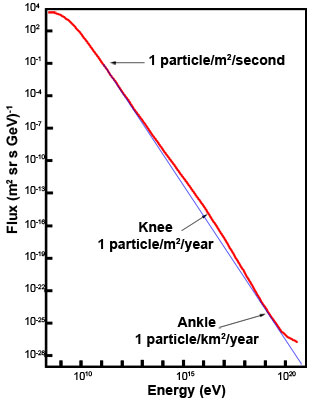
\includegraphics[width=0.35\textwidth]{img/cosmicrayenergies1.jpg}
    \caption{Spettro in energia dei raggi cosmici. Si osservino in particolare i due gomiti dello spettro.}    
    \label{img:cosmicrays}
\end{figure}

\begin{example}
    Proviamo adesso a confrontare le energie dei protoni provenienti dallo spazio che urtano su altri protoni fermi, con le energie dei protoni di LHC. In questo esempio verrà assunto $c = 1$. Supponiamo due protoni che si scontrano, viaggiando in direzione opposta lungo l'asse $\hat{z}$:
    \begin{gather*}
        p_1^\mu = (E^*, 0, 0, \vec{p}), \\
        p_2^\mu = (E^*, 0, 0,  -\vec{p}).
    \end{gather*}
    Dobbiamo confrontare questo caso con quello in cui abbiamo un protone fermo ed uno diretto verso il primo con una certa quantità di moto:
    \begin{gather*}
        p_1'^\mu = (m_\textup{p}, 0, 0, 0), \\
        p_2'^\mu = (E, 0, 0, \vec{p}').
    \end{gather*}
    Sommando semplicemente i primi due 4-vettori, otteniamo che per i protoni nel caso di LHC vale
    \begin{equation*}
        2E^* = E_\textup{cm} \simeq 10^13\,\textup{eV}.
    \end{equation*}
    Per i protoni nel secondo caso abbiamo invece
    \begin{equation*}
        \begin{split}
            (p_1'^\mu + p_2'^\mu)^2 & = (p_1'^\mu)^2 + (p_2'^\mu)^2 + p_1'^\mu \cdot p_2'_\mu \\
                                    & \simeq 2Em_\textup{p} \\
                                    & \simeq (10^{13}\,\textup{eV})^2,
        \end{split}
    \end{equation*}
    dove l'ultimo passaggio viene assunto valido dal momento in cui si vuole confrontare l'energia dei due processi, abbiamo inoltre trascurato un termine proporzionale a $m_\textup{p}^2$. Si ricava dunque
    \begin{equation*}
        E \simeq \frac{(10^{13}\,\textup{eV})^2}{2m_\textup{p}} \simeq 5 \times 10^{16}\,\textup{eV}.
    \end{equation*}
    Questa è l'energia che deve avere un protone proveniente dallo spazio che, urtando su un protone fermo presente nell'atmosfera, dà un'energia nel centro di massa pari a quella di LHC. Confrontando questa informazione con il grafico in figura Fig.(\ref{img:cosmicrays}) vediamo che gli esperimenti condotti ad LHC ci permettono di concludere osservazioni su particelle provenienti da raggi cosmici che corrispondono ad energie nell'intorno del primo ginocchio del grafico.
\end{example}

Con il progredire delle misure fatte sugli sciami cosmici, si sono osservati anche gli andamenti dei flussi in funzione del numero atomico $Z$: in particolare si è osservato come la composizione dei raggi cosmici comprendesse tutti i nuclei fino al Fe per poi fermarsi. In figura Fig.(\ref{img:cosmicZ}) si riporta l'andamento di tali flussi, in tabella Tab.(\ref{tab:cosmicZ}) si riporta in particolare il flusso relativo a quello di Fig.(\ref{img:cosmicrays}).

\begin{figure}[H]
    \centering
    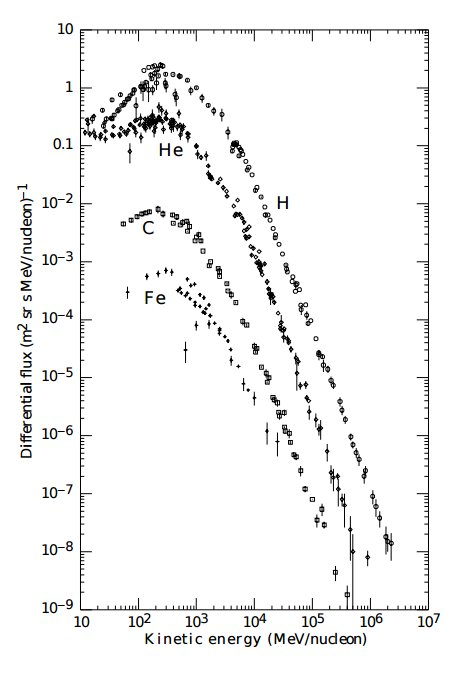
\includegraphics[width=0.4\textwidth]{img/cosmicrayZ.jpg}
    \caption{Andamento dei flussi per diversi nuclei.}  
    \label{img:cosmicZ}  
\end{figure}

\begin{table}[H]
    \centering
    \begin{tabular}{lll}
        \toprule
        \textbf{Z} & \textbf{Elemento} & \textbf{Flusso relativo} \\
        \midrule
        1          & H                 & 540                      \\
        2          & He                & 26                       \\
        3-5        & Li-B              & 0.40                     \\
        6-8        & C-O               & 2.20                     \\
        9-10       & F-Ne              & 0.30                     \\
        \bottomrule
    \end{tabular}
    \caption{Valori di flusso relativo per i nuclei che compongono i raggi cosmici, in rapporto al flusso totale misurato.}
    \label{tab:cosmicZ}
\end{table}

Inoltre sappiamo che:
\begin{itemize}
    \item il flusso di elettroni è circa due ordini di grandezza inferiore a quello dei protoni,
    \item il flusso di positroni è circa $1/20$ di quello degli elettroni,
    \item il flusso di antiprotoni è circa $10^{-4}$ di quello dei protoni.
\end{itemize}
Osservazioni negli anni del flusso di protoni mostrano che la componente a bassa energia nello spettro del flusso di protoni dallo spazio cambia nel tempo: questo è presumibilmente legato all'attività magnetica solare. Non ci sono variazioni nella parte di flusso ad alta energia ($\gtrsim 1\,\textup{GeV}$).

\section{Richiami di perdita di energia delle particelle nella materia}\index{Perdita di energia nella materia}

L'interazione fra particelle e la materia viene classificata sulla base della carica e della massa (al solito, i neutrini
fanno storia a sè). Quando parliamo di particelle pesanti cariche (tipicamente adroni), vogliamo studiare il loro passaggio nella materia: nelle condizioni più comuni ($m \gg m_\textup{e}$, piccolo impulso trasferito, elettrone atomico libero e in quiete) possiamo parlare di ionizzazione del materiale. La grandezza di interesse è $-\der E / \der x$, questa segue la nota formula di Bethe-Block:
\begin{equation*}
    -\frac{\der E}{\der x} = 2\pi N_\textup{A} r_\textup{e}^2 m_\textup{e} c^2 \frac{Z}{A} \frac{^2}{\beta} \biggl[ \ln \frac{2m_\textup{e}c^2 \gamma^2 \beta^2 W_\textup{max}}{I^2} 2\beta^2 - \delta - 2\frac{C}{Z}\biggr].
\end{equation*}
Questa formula descrive la perdita di energia per ionizzazione del mezzo in funzione della \emph{lunghezza ridotta} $x = L\rho$, essendo $\rho$ la densità del mezzo. La perdita di energia viene chiamata anche \emph{stopping power} del mezzo attraversato.

Gli elettroni non perdono energia nella stessa maniera delle altre particelle. Ci sono due meccanismi principali con cui gli elettroni perdono energia:
\begin{itemize}
    \item Collisione atomiche (ionizzazione), in questo caso vale il seguente andamento:
    \begin{equation*}
        -\frac{\der E}{\der x} \biggr|_\textup{Coll} \varpropto Z \ln E_0,
    \end{equation*}
    \item Bremmtrahlung, in questo caso vengono emessi fotoni nel campo di un nucleo
    \begin{equation*}
        -\frac{\der E}{\der x} \biggr|_\textup{Brem} \varpropto Z^2 E_0.
    \end{equation*}
\end{itemize}
Ciascuno dei due processi domina sull'altro a diverse scale di energia.
\begin{definition}[Energia critica]
    L'energia a cui i due processi si equivalgono viene definita con il nome di \emph{energia critica}, empiricamente è descritta dalla seguente formula:
    \begin{equation*}
        E_\textup{C} \approx \frac{800\,\textup{MeV}}{Z + 1}.
    \end{equation*}
    Al di sopra dell'energia critica, la perdita di energia dovuta al processo di Bremmstrahlung è maggiore di quella per ionizzazione.
\end{definition}

I fotoni hanno vari meccanismi di perdita di energia, i tre più importanti sono i seguenti:
\begin{itemize}
    \item effetto fotoelettrico a basse energie ($\lesssim 1\,\textup{keV}$), $\sigma \varpropto Z^5$,
    \item scattering Compton a energie intermedie ($\simeq 1\,\textup{MeV}$), $\sigma \varpropto Z$,
    \item produzione di coppie ad alte energie ($E_\gamma \geqslant 2m_\textup{e}c^2$, dominante per $E > 20\,\textup{MeV}$), $\sigma \varpropto Z(Z+1)$.
\end{itemize}

\subsection*{Calorimetria}

Quando un fotone o un elettrone con elevata energia urta contro un materiale, si dà orignie ad uno \emph{sciame elettromagnetico} (che differisce da quello \emph{adronico}, ne parleremo più avanti). I processi dominanti sono quelli di Bremmstrahlung e produzione di coppie, gli elettroni e fotoni urtando con i centri scatteranti del materiale attraversato originano altri elettroni e fotoni secondari, il processo si può ripetere un certo numero di volte. Volendo caratterizzare l'intensità dello sciame possiamo scrivere:
\begin{equation}
    I = I_0e^{-x/X_0}   \begin{cases}
                            e^- N \rightarrow e^- N \gamma, \quad X_0 \\
                            \gamma N \rightarrow N e^+ e^-, \quad \frac{9}{7}X_0
                        \end{cases}. 
    \label{eq:intensita_X0}      
\end{equation}
\begin{definition}[Lunghezza di radiazione]
    Si definisce \emph{lunghezza di radiazione} la quantità $X_0$, definita come la distanza media (in cm) che un elettrone deve percorrere nel materiale per ridurre la sua energia di un fattore $1/e$ solo per effetto della radiazione. Per la lunghezza di radiazione vale la seguente formula:
    \begin{equation*}
        \frac{1}{X_0} = 4\alpha r_\textup{e}^2\frac{N_\textup{A}}{A} \bigl\{ Z^2\left[L_\textup{rad} - f(Z)\right] + ZL_\textup{rad}'\bigr\}. 
    \end{equation*}
    Da Eq.(\ref{eq:intensita_X0}) si osservi che la lunghezza in cui i fotoni compiono una produzione di coppia equivale a circa i $\frac{9}{7}X_0$, questa lunghezza è anche chiamata \emph{cammino libero medio} per il processo di produzione di coppie.
\end{definition}

Possiamo modellizzare l'evoluzione di uno sciame elettromagnetico osservando che circa ogni $X_0$ vengono prodotte due nuove particelle a partire da una singola particella, inoltre il processo si ripete fino a quando $E > E_\textup{c}$, in particolare dopo $nX_0$ lunghezza ho $2^n$ particelle:
\begin{gather*}
    E_\textup{p}   = \frac{E_0}{2^n},\\
    E_\textup{c}   = \frac{E_0}{2^{n_\textup{max}}} = E_{\textup{n}_\textup{max}},\\
    n_\textup{max} = \ln \frac{E_0}{E_\textup{c}} \frac{1}{\ln 2}.
\end{gather*}
Secondo il modello precendente, l'energia non viene rilasciata prima di $n_\textup{max}$, dove invece viene rilasciata tutta insieme. Chiaramente lo sviluppo reale è più complesso di così ma qualitativamente si può dire che:
\begin{itemize}
    \item l'andamento iniziale della curva ha un andamento molto veloce dovuto alla \emph{moltiplicazione} delle particelle nello sciame,
    \item si arriva ad un massimo quando le coppie secondarie hanno energia $E_\textup{c}$,
    \item dopo quel punto non c'è più moltiplicazione nello sciame e c'è una discesa lenta,
    \item le dimensioni longitudinali dello sciame crescono logaritmicamente con $E_0$.
\end{itemize}

Quando parliamo di sciami adronici invece, è bene ricordare quali sono i due meccanismi principali di perdita di energia:
\begin{itemize}
    \item interazioni degli adroni con gli elettroni del materiale, dunque perdita di energia per ionizzazione,
    \item interazione degli adroni con il nucleo atomico, dunque urto anelastico con il nucleo con conseguente produzione di adroni leggeri ($\pi^0$ e $\pi^\pm$).
\end{itemize}
Ricordiamo adesso alcune formule utili che ci permettono di schematizzare la \emph{lunghezza di interazione adronica}:
\begin{gather*}
    r_\textup{N} \sim r_\textup{f} \times \sqrt[3]{A}, \\
    \sigma_\textup{N} \varpropto r_\textup{N}^2 \varpropto A^{\frac{2}{3}}, \\
    \lambda_\textup{I} = \frac{1}{\rho_\textup{B}\sigma} \varpropto A^{\frac{1}{3}} \varpropto r_\textup{N}.
\end{gather*}
Gli adroni, in quanto tali, danno vita a sciami che differiscono per alcune caratteristiche da quelli elettromagnetici:
\begin{itemize}
    \item le dimensioni longitudinali e trasversali sono diverse,
    \item la componente \textit{em} prodotta dal decadimneto dei $\pi^0$ è soggetta a forti fluttuazioni, ma in generale varia con l'energia della particella iniziale.
    \item c'è una certa frazione di energia invisibile, dovuta alla presenza di $\nu$ e $\mu$,
    \item i neutroni prodotti durante l'urto anelastico vengono termalizzati e riassorbiti con un certo ritardo.
\end{itemize}
Lo strumento per eccellenza per campionare la perdita di energia (per ionizzazione) nella materia è il \emph{calorimetro}. Questo può essere costruito in vari modi: si classificano per scopo (elettromagnetici o adronici), materiale (gas, di scintillazione, cristalli, liquidi...), composizione (omogenei o a \emph{sampling}) e modalità di lettura (compensazione, double-readout, PFA).

\subsection*{Effetto Cherenkov}

Una particella carica che si muove in un mezzo dielettrico emette onde elettromagnetiche che si propagano a velocità $c/n$, con $n$ indice di rifrazione del mezzo. Se la particella che si propaga nel mezzo ha velocità maggiore di quella nella luce nello stesso mezzo si ha una emissione di un fronte d'onda coerente con un determinato angolo di inclinazione rispetto alla direzione di propagazione della particella. 

\begin{figure}[H]  
    \centering
    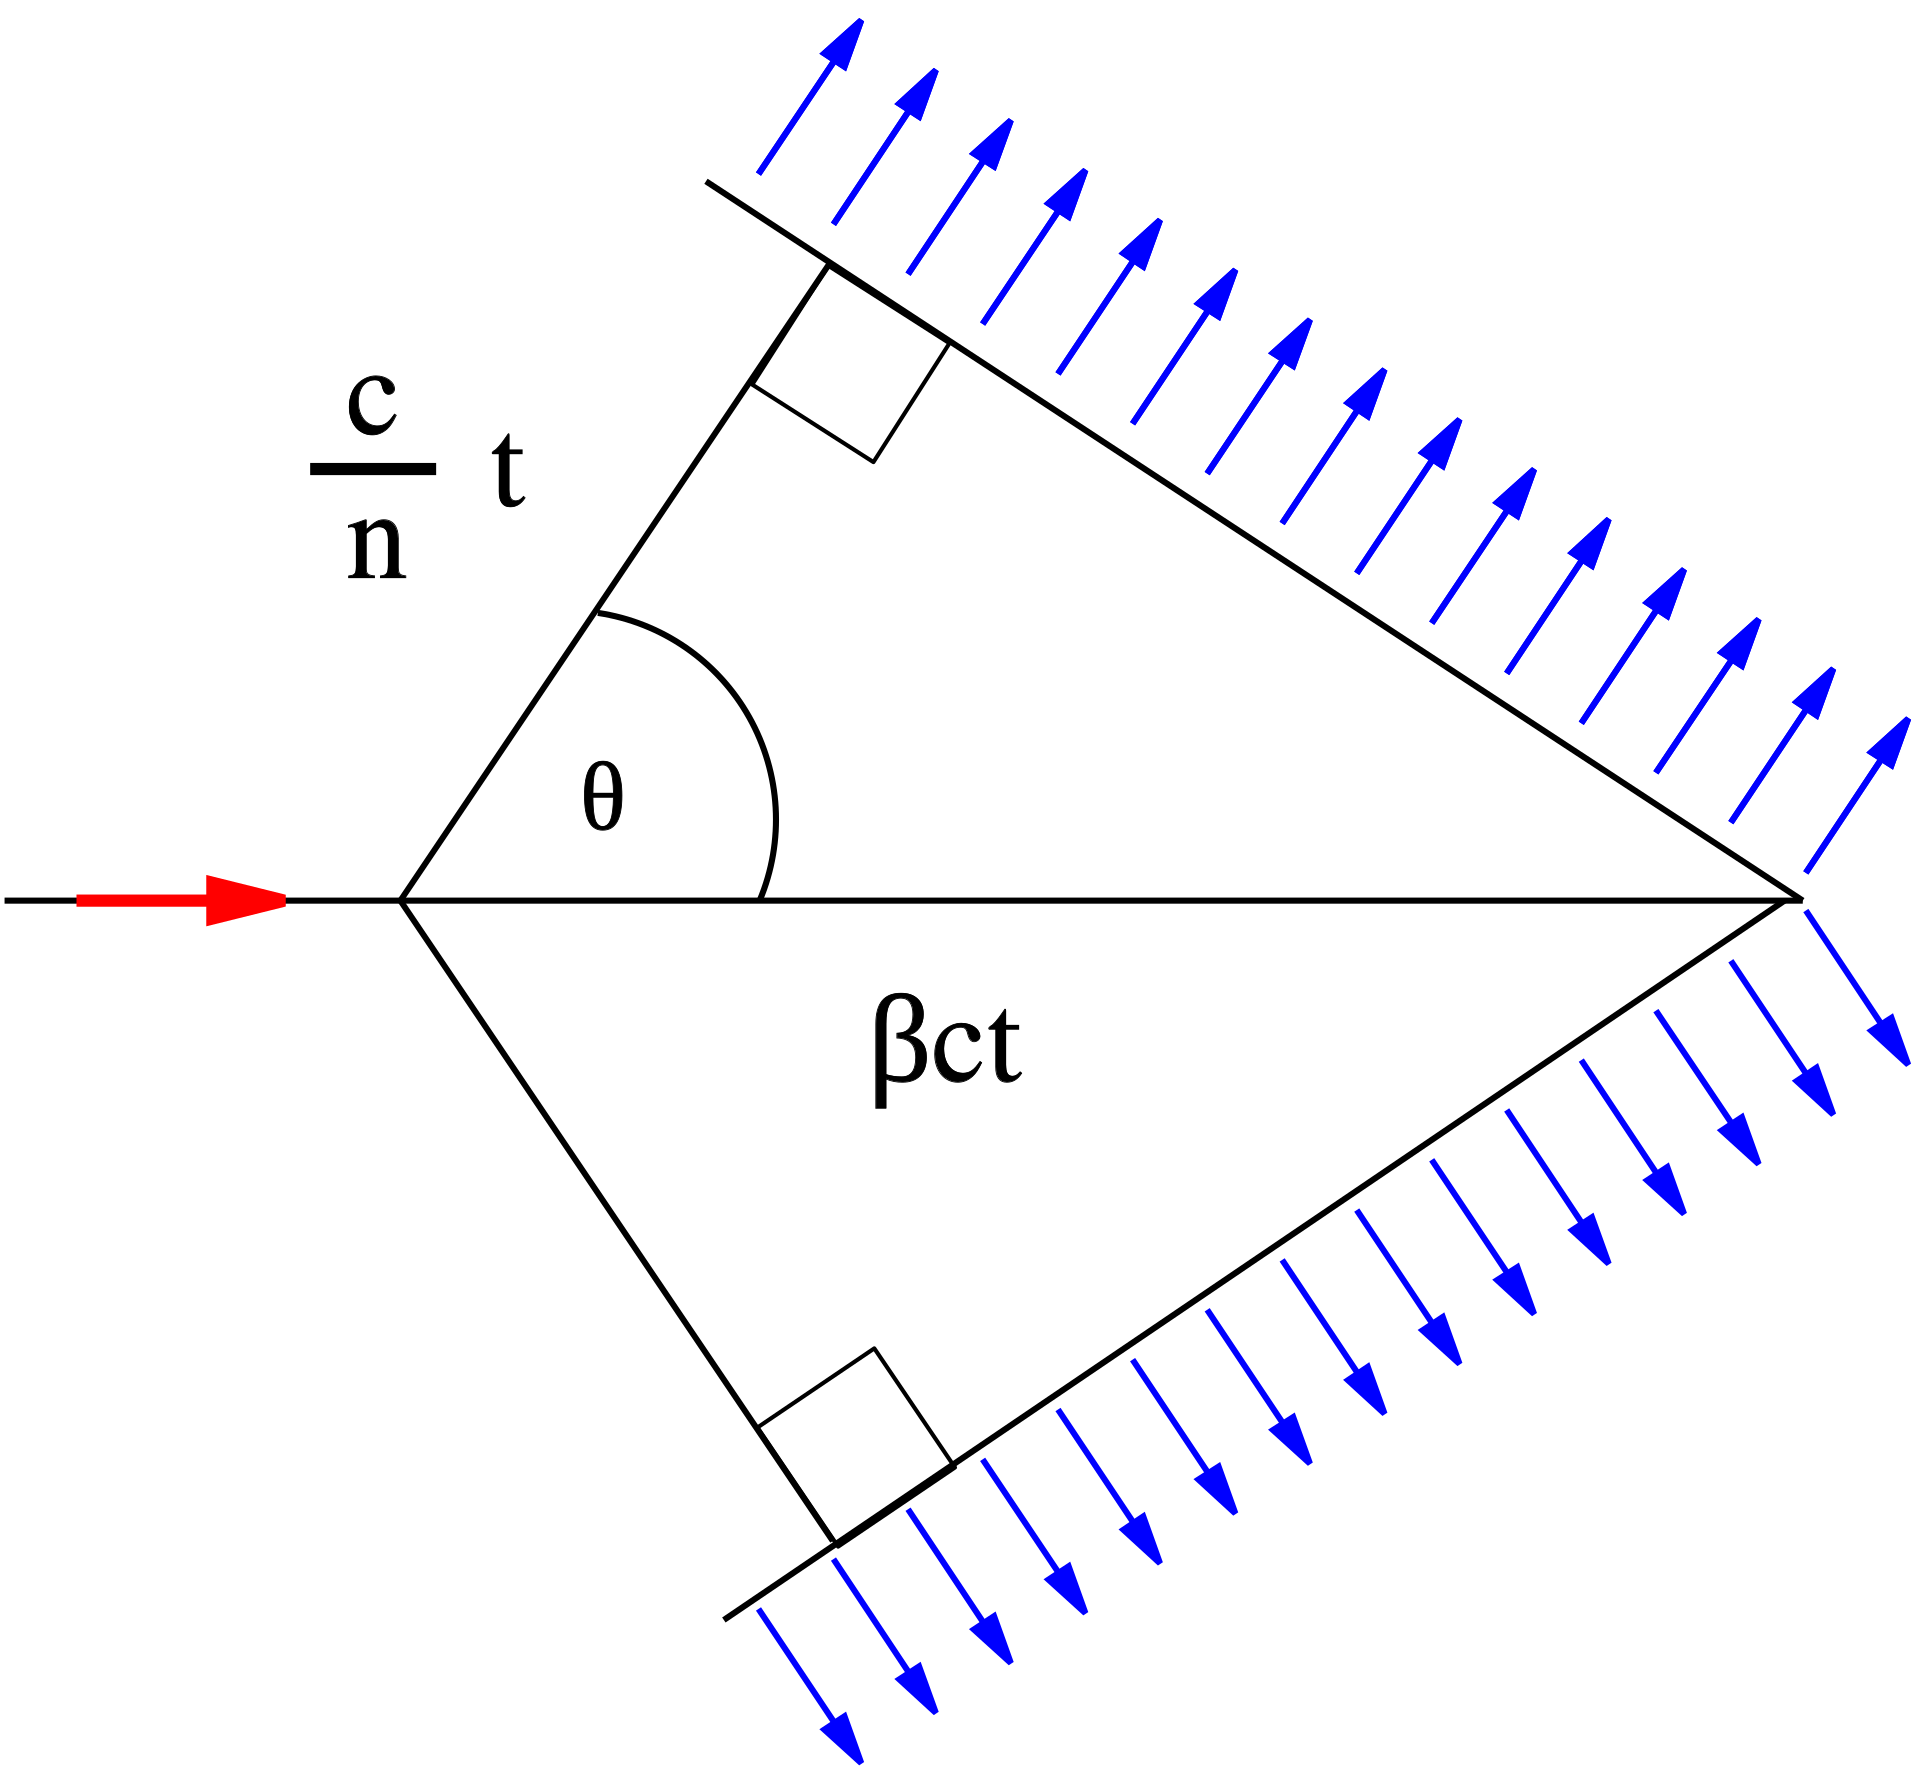
\includegraphics[width=0.4\textwidth]{img/cherenkov_effect.png}
    \caption{Schematizzazione geometrica dell'effetto Cherenkov. In rosso si indica la direzione di propagazione della particella, in blu la direzione del fronte d'onda.}
    \label{img:cherenkov_effect}
\end{figure}
Come si evince dalla figura Fig.(\ref{img:cherenkov_effect}), possiamo scrivere la relazione tra l'angolo $\theta$ e la velocità $\beta$ della particella:
\begin{equation*}
    \cos \theta = \frac{1}{n\beta}.
\end{equation*}
Dall'informazione sul cono di luce emesso possiamo inferire informazioni sulla direzione della particella. Un altro punto fondamentale dell'effetto Cherenkov è che fa da soglia, in quanto l'emissione avviene solo se vale $\beta > 1/n$. Combinando questa informazione con quella della massa della particella posso stimare l'energia della particella (usando la nota relazione $E = m\gamma c^2$).